%!TEX program = xelatex

\documentclass[a4paper, openany, oneside]{memoir}
\usepackage[no-math]{fontspec}
\usepackage{pgfplots}
\usepackage{float}
\pgfplotsset{compat=newest}
\usepackage{commath}
\usepackage{mathtools}
\usepackage{amssymb}
\usepackage{amsthm}
\usepackage{booktabs}
\usepackage{todonotes}
\usepackage{mathtools}
\usepackage{xcolor}
\usepackage[separate-uncertainty=true, per-mode=symbol]{siunitx}
\usepackage{listings}
\usepackage[american inductor, european resistor]{circuitikz}
\usepackage{amsmath}
\usepackage{amsfonts}
\usepackage{ifxetex}
\usepackage[dutch,english]{babel}
\usepackage[backend=bibtexu,texencoding=utf8,bibencoding=utf8,style=ieee,sortlocale=en_GB,language=auto]{biblatex}
\usepackage[strict,autostyle]{csquotes}
\usepackage{import}
\usepackage{standalone}
\usepackage{bookmark,hyperref}
\usepackage{xcolor,mdframed}
\usepackage{tikz}
\usepackage{framed}
\usepackage{float}
\usepackage{tabularx}
\usepackage{graphicx,adjustbox}
\usepackage{rotating}
\usepackage{pdfpages}
\usepackage{enumitem}
\usepackage{calc}
\usepackage{pgfplots}
\usepackage{filecontents}
\usepackage{caption}
\usepackage{subcaption}
\usepackage{lettrine}

\newcolumntype{Y}{>{\raggedright\arraybackslash}X} % Left-justified text in tabularx environment

\ifxetex{} % Fonts laden in het geval dat je met Xetex compiled
    \usepackage{fontspec}
    \defaultfontfeatures{Scale=MatchLowercase, Ligatures=TeX} % To support LaTeX quoting style
    %\setromanfont{Palatino Linotype} % Tover ergens in Font mapje in root.
    \setsansfont{Avenir Next LT Pro}
    \setromanfont{Adobe Caslon Pro} % Tover ergens in Font mapje in root.
    \setmonofont{Source Code Pro}
\else % Terug val in standaard pdflatex tool chain. Geen ondersteuning voor OTT fonts
    \usepackage[T1]{fontenc}
    \usepackage[utf8]{inputenc}
\fi
\usepackage[noabbrev, capitalize]{cleveref}
\usepackage{ifthen}
\usepackage{titlesec}
\usepackage{titlecaps}

\newcommand{\references}[1]{\begin{flushright}{#1}\end{flushright}}
\renewcommand{\vec}[1]{\boldsymbol{\mathbf{#1}}}
\newcommand{\uvec}[1]{\boldsymbol{\hat{\vec{#1}}}}
\newcommand{\mat}[1]{\boldsymbol{\mathbf{#1}}}
\newcommand{\fasor}[1]{\boldsymbol{\tilde{\vec{#1}}}}
\newcommand{\cmplx}[0]{\mathrm{j}}
\renewcommand{\Re}[0]{\operatorname{Re}}
\newcommand{\Cov}{\operatorname{Cov}}
\newcommand{\Var}{\operatorname{Var}}
\newcommand{\proj}{\operatorname{proj}}
\newcommand{\Perp}{\operatorname{perp}}
\newcommand{\col}{\operatorname{col}}
\newcommand{\rect}{\operatorname{rect}}
\newcommand{\sinc}{\operatorname{sinc}}
\newcommand{\lcm}{\operatorname{lcm}}
%\newcommand{\gcd}{\operatorname{gcd}}
\newcommand{\F}{\mathcal{F}}
\newcommand{\DTFT}{\mathcal{F}_*}
\newcommand{\conj}[1]{#1^*}
\renewcommand{\mod}{\operatorname{mod}}
\newcommand{\rot}{\operatorname{rot}}
\newcommand{\vecsc}[1]{\vec{\textsc{\textbf{#1}}}}
\renewcommand{\ss}[1]{_{#1}}

% Label without linebreak breaker
\newcommand{\lab}[1]{\label{#1}\nolinebreak}

\newtheorem{definition}{Definition}
\newtheorem{theorem}{Theorem}


\DeclareSIUnit{\voltampere}{VA} %apparent power
\DeclareSIUnit{\pii}{\ensuremath{\pi}}

\hypersetup{%setup hyperlinks
    colorlinks,
    citecolor=black,
    filecolor=black,
    linkcolor=black,
    urlcolor=black
}

% Example boxes
\usepackage{fancybox}
\usepackage{framed}
\usepackage{adjustbox}
\newenvironment{simpages}%
{\AtBeginEnvironment{itemize}{\parskip=0pt\parsep=0pt\partopsep=0pt}
\def\FrameCommand{\fboxsep=.5\FrameSep\shadowbox}\MakeFramed{\FrameRestore}}%
{\endMakeFramed}

% Impulse train
\DeclareFontFamily{U}{wncy}{}
\DeclareFontShape{U}{wncy}{m}{n}{<->wncyr10}{}
\DeclareSymbolFont{mcy}{U}{wncy}{m}{n}
\DeclareMathSymbol{\Sha}{\mathord}{mcy}{"58}

\setlength{\parindent}{0pt}
\nonzeroparskip

% Block environment configuration
\newcommand{\BlockLeftMargin}{20pt}
\newcommand{\BlockLeftMarginText}{25pt}
\newcommand{\BlockLeftMarginTextSpacing}{10pt}

% Own colours
\definecolor{gray75}{gray}{0.75}

% Block environment
\newenvironment{block}[3]{%
\makebox{\hspace{-\spinemargin}%
\begin{tikzpicture}[overlay]
    \draw [thick,color=gray75] (\BlockLeftMargin, 0) -- (\paperwidth - \spinemargin, 0);
    \node at (\BlockLeftMarginText, -0.9) [align=left, text width=\spinemargin - \BlockLeftMarginText - \BlockLeftMarginTextSpacing, anchor=west, text depth=1cm] {\textbf{\textsc{#1}}\newline\textit{#3}};
\end{tikzpicture}}%
\nopagebreak\\[0.25em]\ifthenelse{\equal{#2}{}}{}{(\textit{#2}.) }\nopagebreak\nolinebreak}
{\nopagebreak\\[-0.25em]%
\makebox{\hspace{-\spinemargin}%
\begin{tikzpicture}[overlay, remember picture]
    \draw [thick,color=gray75] (\spinemargin,0) -- (\paperwidth - \spinemargin,0);
\end{tikzpicture}} \vspace{0.5em}}

% Theorem
\newcounter{blockTheoremCounter}
\crefname{blockTheoremCounter}{Theorem}{Theorems}
\Crefname{blockTheoremCounter}{Theorem}{Theorems}

\newenvironment{blockTheorem}[1][]{%
\refstepcounter{blockTheoremCounter}%
\begin{block}{theorem \theblockTheoremCounter}{#1}{}}
{\end{block}}

% Definition
\newcounter{blockDefinitionCounter}
\crefname{blockDefinitionCounter}{Definition}{Definitions}
\Crefname{blockDefinitionCounter}{Definition}{Definitions}

\newenvironment{blockDefinition}[1][]{%
\refstepcounter{blockDefinitionCounter}%
\begin{block}{definition \theblockDefinitionCounter}{#1}{}}
{\end{block}}

% Proof
\newcounter{blockProofTheoremCounter}
\crefname{blockProofTheoremCounter}{Proof}{Proofs}
\Crefname{blockProofTheoremCounter}{Proof}{Proofs}

\newenvironment{blockProofTheorem}[1]{%
\refstepcounter{blockProofTheoremCounter}%
\begin{block}{proof of \\ theorem #1}{}{}}
{\qed\end{block}}

% Detail
\newcounter{blockDetailCounter}
\crefname{blockDetailCounter}{Detail}{Details}
\Crefname{blockDetailCounter}{Detail}{Details}

\newenvironment{blockDetail}[1][]{%
\refstepcounter{blockDetailCounter}%
\begin{block}{detail \theblockDetailCounter}{#1}{}}
{\end{block}}

% Redesign chapter headings
\newcommand{\chapternumber}{\thechapter}
\newcommand{\hsp}{\hspace{20pt}}
\titleformat{\chapter}[hang]{\Huge\bfseries}{\chapternumber\hsp\textcolor{gray75}{|}\hsp}{0pt}{\Huge\bfseries}

% Remove headers
% \addtopsmarks{headings}{}{
%   \createmark{chapter}{left}{nonumber}{}{}
% }
% \pagestyle{headings} % Activate changes

% Capitalise headers in a regular way
\renewcommand*{\memUChead}[1]{\titlecap{#1}}

% \hfill for math mode
\newcommand{\pushright}[1]{\intertext{\hfill$\displaystyle #1$}}
\newcommand{\pushline}{\hskip \textwidth minus \textwidth}
\newcommand{\matlab}{\textsc{Matlab}}

\definecolor{code-grey}{HTML}{DDDDDD}
\newcommand{\lib}[1]{\textsf{#1}}
\newcommand{\file}[1]{\textsf{#1}}
\newcommand{\func}[1]{\colorbox{code-grey}{\texttt{#1}}}
\newcommand{\class}[1]{\colorbox{code-grey}{\texttt{#1}}}

% Setup actiepunten
\newenvironment{important}[1][]{%
   \begin{mdframed}[%
      backgroundcolor={red!15}, hidealllines=true,
      skipabove=0.7\baselineskip, skipbelow=0.7\baselineskip,
      splitbottomskip=2pt, splittopskip=4pt, #1]%
   \makebox[0pt]{% ignore the withd of !
      \smash{% ignor the height of !
         \fontsize{32pt}{32pt}\selectfont% make the ! bigger
         \hspace*{-19pt}% move ! to the left
         \raisebox{-2pt}{% move ! up a little
            {\color{red!70!black}\sffamily\bfseries !}% type the bold red !
         }%
      }%
   }%
}{\end{mdframed}}
\newcommand{\excl}[1]{
\begin{important}
  \textbf{#1}
\end{important}
}

\makeatletter
\newcommand\footnoteref[1]{\protected@xdef\@thefnmark{\ref{#1}}\@footnotemark}
\makeatother

% Allow page breaks in display environments
%\allowdisplaybreaks
% S unit for use in Mega Samples per second
\DeclareSIUnit\sample{S}

\newcommand{\CC}{C\nolinebreak\hspace{-.05em}\raisebox{.3ex}{ \textbf{+}}\nolinebreak\hspace{-.10em}\raisebox{.3ex}{\textbf{+}}}
\def\CC{{C\nolinebreak[4]\hspace{-.05em}\raisebox{.3ex}{\textbf{++}}}}


\newcommand{\partauthor}[1]{\gdef\@partauthor{#1}}
\renewcommand{\printparttitle}[1]{
  \parttitlefont #1\\
  \vspace{1.5cm}
  \textnormal{\Large \@partauthor}
}
\addbibresource{../../../../includes/bibliography.bib}

\begin{document}

\section{Energy detection}
Conventional energy detection is a detection method that measures the energy of a signal $x[n]$, $\Lambda$, during a certain period. By comparing this measured energy to a threshold $\gamma$ the detector decides whether the input signal $x[n]$ contains only noise or that another signal besides noise is present in $x[n]$:

\begin{align*}
	\begin{cases}
		\mathcal{H}_0 & \text{if } \Lambda < \gamma \\
		\mathcal{H}_1 & \text{if } \Lambda > \gamma
	\end{cases}
\end{align*}
 
Given $N$ samples of $x[n]$, the measure of energy, $\Lambda$, which is used as test statistic is given by 

\begin{align}\label{eq:test_ed}
	\Lambda &= \sum_{n=0}^{N-1} |x[n]|^2.
\end{align}

The threshold $\gamma$ depends on the expected noise power $\sigma_n^2$ and the desired false alarm probability $p_{fa}$: the probability that the detector decides that hypothesis 2 is true, while hypothesis 1 is the true hypothesis. The derivation of $\gamma$ (see Appendix ...) gives the following result

\begin{align*}
\gamma = \left[Q^{-1}(p_{fa})\sqrt{N} + N\right]2\sigma_n^2
\end{align*}

where $Q^{-1}$ denotes the the inverse tail probability function of the standard normal distribution and $p_{fa}$ is the desired false alarm probability.
Using a bandpass filter $H(f)$ one can filter the signal $x[n]$ such that it can be used to detect a signal in a particular frequency band. This whole process is depicted
in \cref{tkz:conv_ed}
\begin{figure}[H]
\centering
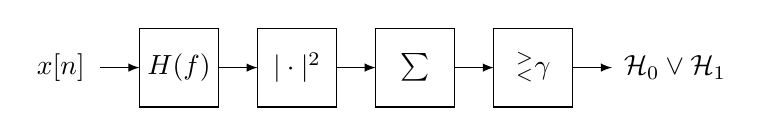
\begin{tikzpicture}

\node at (-6,2) {$x[n]$};
\node at (1.8,2) {$\mathcal{H}_0 \lor \mathcal{H}_1$};

\draw [>=latex, ->] (-5.5,2) -- (-5,2);
\draw (-5,2.5) rectangle (-4,1.5) node[pos=.5]{$H(f)$};

\draw [>=latex, ->] (-4,2) -- (-3.5,2);
\draw (-3.5,2.5) rectangle (-2.5,1.5) node[pos=.5]{$|\cdot|^2$};

\draw [>=latex, ->] (-2.5,2) -- (-2,2);
\draw (-2,2.5) rectangle (-1,1.5) node[pos=.5]{$\sum$};

\draw [>=latex, ->] (-1,2) -- (-0.5,2); 
\draw (-0.5,2.5) rectangle (0.5,1.5) node[pos=.5]{$_<^ > \gamma$};

\draw [>=latex, ->] (0.5,2) -- (1,2);

\end{tikzpicture}
\caption{Conventional Energy Detector}\label{tkz:conv_ed}
\end{figure}

% As can be seen from  \cref{eq:test_ed} the test statistic used by the conventional energy detector does not take into account that the signal to be detected resides in a certain frequency band. Therefore it is necessary that the input signal $x[n]$ is filtered before $\Lambda$ is computed.

As can be noted from \cref{eq:test_ed} the test statistic depends on the signal itself, not on the autocorrelation which serves as input of our detector.
In the rest of this section, we will show how the test statistic can be modified
such that the autocorrelation function can be used to detect the presence of  a signal in a certain frequency band.

Let 
\begin{align*}
\Lambda' &= \frac{\Lambda}{N}\\
	&= \frac{\sum_{n=0}^{N-1} |x[n]|^2}{N},
\end{align*}
then $\Lambda'$ is an estimate of the average power $E\left[|x[n]|^2\right]$ of the signal $x$. We can use $\Lambda'$ as test statistic by using a modified threshold $\gamma' = \frac{\gamma}{N}$. By definition of the power spectral density we know that integral over the power spectral density equals the expected average power:

\begin{align}\label{eq:average_power_psd}
E\left[\left|x[n]\right|^2\right] = \frac{1}{2\pi} \int_{-\pi}^{\pi}\mathcal{P}_x(\omega) \text{d}\omega.
\end{align}
Furthermore, by the Wiener-Khinchin theorem we have that, if $x[n]$ is wide-sense stationary (as is assumed in the reconstructor),
\begin{align}\label{eq:wiener_psd}
	\mathcal{P}_x(\omega) = \sum_{n=-\infty}^{\infty} r_x[n] \exp [2\pi j\omega].
\end{align}
By combining \cref{eq:average_power_psd} and \cref{eq:wiener_psd} we can relate the autocorrelation function to the test statistic $\Lambda'$.
The test statistic $\Lambda'$, however, still does not allow for detection in a certain frequency band.

 Notice that if $x[n]=w[n]$, its autocorrelation function equals a delta function: $r_x[n] = \sigma_n^2\delta[n]$, with $\sigma_n^2$ the average noise power. 
 Therefore the power spectral density of $x[n]$, denoted by $\mathcal{P}(\omega)$ equals  
 \begin{align*}
 \mathcal{P}_x(\omega) = \sum_{n=-\infty}^{\infty}r_x[n]e^{-jn\omega} = \sigma_n^2.
 \end{align*} The power spectral density is constant. If we want to detect the presence of a signal in a certain frequency band $W$, we can make use of this characteristic. Let

 \begin{align*}
 \Lambda'' &= \int_W \mathcal{P}(\omega) \text{d}\omega
 \end{align*}
denote the test statistic to detect a signal in the frequency band W.
 If we would integrate the power spectral density of noise over $W$ we obtain an average power of  $\frac{W}{2\pi} \sigma_n^2$. Therefore if we are to use $\Lambda''$ as test statistic, we have to use the modified threshold $\gamma'' = \frac{W}{2\pi} \gamma'$.

 By applying the fourier transform to the autocorrelation one can use this test statistic to apply the detection process to several frequency bands, as depicted in \cref{tkz:my_ed}.

 \begin{figure}[H]
\centering
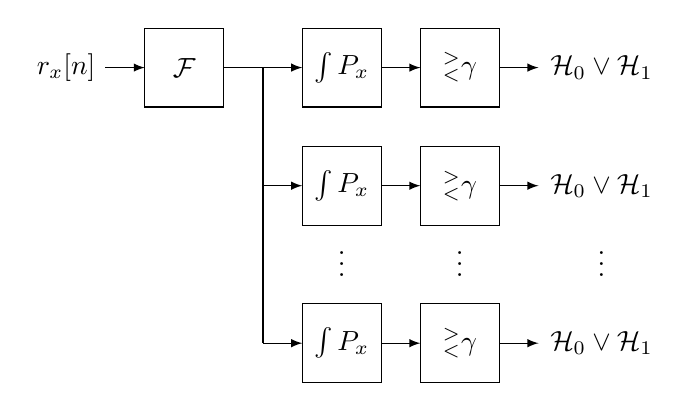
\begin{tikzpicture}

\node at (-6.5,2.5) {$r_x[n]$};

\draw [>=latex, ->] (-6,2.5) -- (-5.5,2.5);
\draw (-5.5,3) rectangle (-4.5,2) node[pos=.5]{$\mathcal{F}$};

\draw [>=latex, ->] (-4.5,2.5) -- (-3.5,2.5);
\draw (-3.5,3) rectangle (-2.5,2) node[pos=.5]{$\int P_x$};

\draw [>=latex, ->] (-2.5,2.5) -- (-2,2.5);
\draw (-2,3) rectangle (-1,2) node[pos=.5]{$_<^ > \gamma$};

\draw [>=latex, ->] (-1,2.5) -- (-0.5,2.5);
\node at (0.3,2.5) {$\mathcal{H}_0 \lor \mathcal{H}_1$};


\draw [>=latex, ->] (-4,1) -- (-3.5,1);
\draw (-3.5,1.5) rectangle (-2.5,0.5) node[pos=.5]{$\int P_x$};

\draw [>=latex, ->] (-2.5,1) -- (-2,1);
\draw (-2,1.5) rectangle (-1,0.5) node[pos=.5]{$_<^ > \gamma$};

\draw [>=latex, ->] (-1,1) -- (-0.5,1);
\node at (0.3,1) {$\mathcal{H}_0 \lor \mathcal{H}_1$};


\draw [>=latex, ->] (-4,-1) -- (-3.5,-1);
\draw (-3.5,-0.5) rectangle (-2.5,-1.5) node[pos=.5]{$\int P_x$};

\draw [>=latex, ->] (-2.5,-1) -- (-2,-1);
\draw (-2,-0.5) rectangle (-1,-1.5) node[pos=.5]{$_<^ > \gamma$};

\draw [>=latex, ->] (-1,-1)-- (-0.5,-1);
\node at (0.3,-1) {$\mathcal{H}_0 \lor \mathcal{H}_1$};

\draw (-4,2.5) -- (-4,-1);


\node at (-3,0.11) {\vdots};
\node at (-1.5,0.11) {\vdots};
\node at (0.3,0.11) {\vdots};

\end{tikzpicture}
\caption{Energy detection, multiple frequency bands}\label{tkz:my_ed}
\end{figure}

Note that this detector depends on the amount of samples $N$ that were used to calculate $\Lambda$. However, this poses a problem if the detector uses the estimated autocorrelation of the reconstructor: what is $N$?

In signal processing the autocorrelation function $r_x[n]$ is usually estimated by 

\begin{equation}\label{eq:acf_est}
r_x[n] = \frac{1}{N-|n|}\sum_{m=\max(0,n)}^{N-1+\min(0,n)} x[m]\overline{x}[m-n]
\end{equation}

By \cref{eq:acf_est} we have that $r_x[0] = \sum_{n=0}^{N-1} |x[n]|^2 = \Lambda$. That is, $N$ should be the amount of samples needed to estimate $r_x[0]$ in case that \cref{eq:acf_est} is used. However, the reconstructor does not use \cref{eq:acf_est}, instead it combines samples from multiple cosets, which obscures what the value of $N$ should be. 

% \subsection{Noise variance}
% As indicated, knowledge of the noise variance is necessary for the energy detector to work. In practical situations this noise variance may be estimated from a reference measurement in an empty frequency band. 
\subsection{Energy detection with knowledge of the reconstructor}
The problem with the conventional energy detector described above is that the parameter $N$ is not straightforward to determine. The energy detector as described in \cite{ariananda2012compressive} uses the power spectral density as test statistic. The power spectral density is estimated by applying the Discrete Fourier Transform to the estimate of the autocorrelation function. With a frequency specific threshold, $\gamma_{\omega}$, the detector decides per frequency whether $\mathcal{H}_0$ or $\mathcal{H}_1$ is true, as can be seen from \cref{tkz:ed_ari_overview}. This detector can actually be regarded as the detector in \cref{tkz:my_ed} where the discrete power spectral density used and $W=\frac{2\pi}{2LN+1}$.  

\begin{figure}[H]
\centering
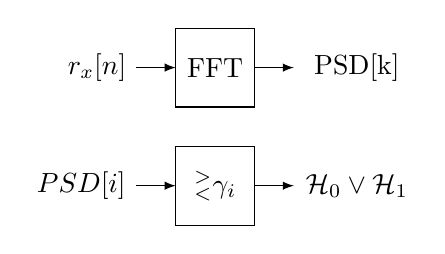
\begin{tikzpicture}

\node at (-3,4) {$r_x[n]$};

\draw [>=latex, ->] (-2.5,4) -- (-2,4);

\draw (-2,4.5) rectangle (-1,3.5) node[pos=.5]{FFT};

\draw [>=latex, ->] (-1,4) -- (-0.5,4);
\node at (0.3,4) {PSD[k]};

\node at (-3.2,2.5) {$PSD[i]$};

\draw [>=latex, ->] (-2.5,2.5) -- (-2,2.5);

\draw (-2,3) rectangle (-1,2) node[pos=.5]{$_<^ > \gamma_i$};

\draw [>=latex, ->] (-1,2.5) -- (-0.5,2.5);
\node at (0.3,2.5) {$\mathcal{H}_0 \lor \mathcal{H}_1$};

\end{tikzpicture}
\caption{Energy detection with knowledge of the reconstructor}\label{tkz:ed_ari_overview}
\end{figure}

 To determine the threshold $\gamma_{\omega}$ for each element, the signal $x[n]$ is assumed to contain purely additive circular complex gaussian noise. The distribution of the elements of the reconstructed power spectral density is then approximated as a normal distribution, see Appendix \textbf{TODO} for a derivation.

\begin{figure}[H]
\centering
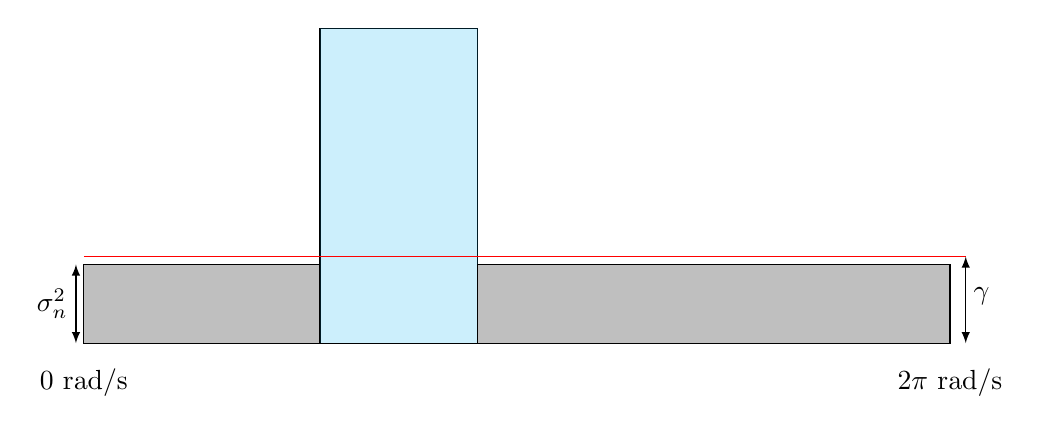
\begin{tikzpicture}

\draw [fill=lightgray] (-2,0) rectangle (1,-1);
\draw (1,3) rectangle (3,-1);
\draw [fill=cyan, opacity=0.2] (1,3) rectangle (3,-1);
\draw [fill=lightgray](3,0) rectangle (9,-1);


\draw [>=latex,<->] (-2.1,-1) -- (-2.1,0);
\node at (-2.4,-.5) {$\sigma^2_n$};

\draw [red] (-2,.1) -- (9.2,.1);

\draw [>=latex,<->] (9.2,-1) -- (9.2,.1);
\node at (9.4,-.4 ) {$\gamma$};

\node at (-2,-1.5) {0 rad/s};
\node at (9,-1.5) {$2\pi$ rad/s};
\end{tikzpicture}
\caption{Energy detection with power spectral density}\label{tkz:ed_ari}
\end{figure}

Given $\mu (\omega) = E[\mathcal{P}(\omega)]$ and $\sigma^2 (\omega) = \text{Var}(\mathcal{P}(\omega))$, a threshold for each frequency $\omega$ given a false alarm probability can be calculated as:

\begin{align*}
\gamma(\omega) &= Q^{-1}(p_{fa})\sigma (\omega) + \mu (\omega) 
\end{align*}

%  \subsection{Determining $\mu(\omega)$ and $\sigma^2(\omega)$}
% In this section we will describe how $\mu(\omega$ and $\sigma^2(\omega)$ can be derived given a reconstructed autocorrelation.

% Let $\mat{F}$ denote the $(2NL+1) \times (2NL+1) $ DFT matrix, then
% \begin{align*}
% \vec{s}_x = \mat{F}\mat{R}^{\dagger}\vec{r}_y
% \end{align*}
% denotes the vector containing the elements of the reconstructed power spectral density of $x[n]$. That is the element $\left(\vec{s}_{x}\right)_{i}$ denotes the component of the power spectral density at $\omega = \frac{2\pi (i-1)}{2LN-1}$.

% To obtain $\text{Var}(\vec{s}_x)_i$ for each element in $\vec{s}_x$, we compute the covariance matrix $\mat{C}_{s_x}$ of $\vec{s}_x$ as 

% \begin{align*}
% 	\mat{C}_{s_x} &= E\left[\vec{s}\vec{s}^H\right] - E\left[\vec{s}\right]E\left[\vec{s}^H\right]
% \end{align*} 

% The variance $\sigma^2$ of the elements of $\vec{s}_x$ will then given by the diagonal of $\mat{C}_{s_x}$.
% We can express $\mat{C}_{s_x}$ as

% \begin{align*}
% \mat{C}_{s_x} &= E\left[\vec{s}_x\vec{s}_x^H\right] - E\left[\vec{s}\right]E\left[\vec{s}^H\right] \\
% &= E\left[\left(\mat{F} \mat{R}^{\dagger}\vec{r}_y\right) \left( \mat{F}\mat{R}^{\dagger}\vec{r}_y\right)^H\right] - E\left[\mat{F}\mat{R}^{\dagger}\vec{r}_y\right]E\left[\left(\mat{F}\mat{R}^{\dagger}\vec{r}_y\right)^H\right] \\
% &= \mat{F}\mat{R}^{\dagger} E\left[ \vec{r}_y\vec{r}_y^H\right]  \mat{R}^{\dagger H}\mat{F}^H -  \mat{F}\mat{R}^{\dagger} E\left[ \vec{r}_y\right] E\left[\vec{r}_y^H\right]   \mat{R}^{\dagger H}\mat{F}^H \\
% &= \mat{F}\mat{R}^{\dagger} \mat{C}_{r_y} \mat{R}^{\dagger H}\mat{F}^H.
% \end{align*}

% $\mat{C}_{r_y}$ denotes the covariance matrix of $\vec{r}_y$ and is defined as

% \begin{align*}
%  E\left[\vec{r}_y\vec{r}_y^H\right] - E\left[\vec{r}_y\right]E\left[\vec{r}_y^H\right]
% \end{align*}

% In case that $x[n]$ contains white noise with variance $\sigma_n$, the elements of $\mat{C}_{r_y}$ are given by

% \begin{align*}
% \text{Cov}\left(r_{y_r,y_s}[t],r_{y_u,y_v}[w]\right) &= \sigma_n^4 r_{c_r,c_u}[0]r_{c_s,c_v}[0]\delta[w-t]
% \end{align*}

% That is, by computing the theoretical covariance $C_{r_y}$ in the case that $x[n]$ contains only noise, we can compute $\mat{C}_{s_x}$.
% By taking the diagonal of $\mat{C}_{s_x}$ we obtain the vector $[\sigma^2(\frac{2\pi k}{d} $

\section{Covariance absolute value method}
The covariance absolute value detection method as introduced does \emph{not} depend on the noise power. Its test statistic is based on the structure of the autocorrelation function $r_x[n]$. 

\begin{figure}[H]
\centering
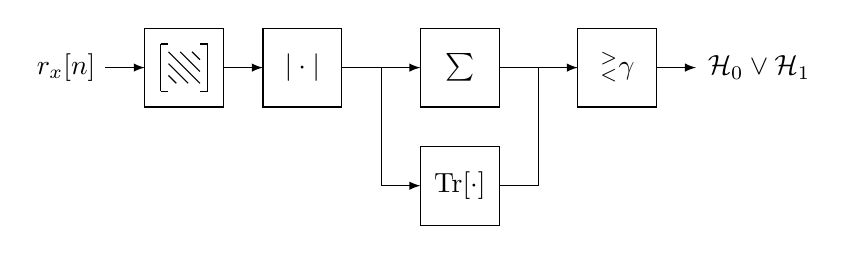
\begin{tikzpicture}

\node at (-4,4.5) {$r_x[n]$};

\draw [>=latex, ->] (-3.5,4.5) -- (-3,4.5);

\draw (-3,5) rectangle (-2,4) node[pos=.5]{};
\draw [>=latex, ->] (-2,4.5) -- (-1.5,4.5);

\draw (-1.5,5) rectangle (-0.5,4) node[pos=.5]{$|\cdot|$};
\draw [>=latex, ->] (-0.5,4.5) -- (0.5,4.5);

\draw (2.5,5) rectangle (3.5,4) node[pos=.5]{$_<^ > \gamma$};
\draw [>=latex, ->] (3.5,4.5) -- (4,4.5);

\draw (0.5,5) rectangle (1.5,4) node[pos=.5]{$\sum$};
\draw [>=latex, ->] (1.5,4.5) -- (2.5,4.5);

\draw (0.5,3.5) rectangle (1.5,2.5) node[pos=.5]{Tr[$\cdot$]};

\node at (4.8,4.5) {$\mathcal{H}_0 \lor \mathcal{H}_1$};

\draw (0,4.5) -- (0,3);
\draw (2,4.5) -- (2,3);
\draw (2,3) -- (1.5,3);
\draw [>=latex,->] (0,3) -- (0.5,3);

\draw (-2.6,4.3) -- (-2.7,4.4);

\draw (-2.45,4.3) -- (-2.7,4.55);
\draw (-2.3,4.3) -- (-2.7,4.7);
\draw (-2.3,4.45) -- (-2.55,4.7);

\draw (-2.3,4.6) -- (-2.4,4.7);

\draw (-2.8,4.8) -- (-2.8,4.2);
\draw (-2.8,4.8) -- (-2.7,4.8);
\draw (-2.8,4.2) -- (-2.7,4.2);

\draw (-2.2,4.8) -- (-2.2,4.2);
\draw (-2.2,4.2) -- (-2.3,4.2);
\draw (-2.2,4.8) -- (-2.3,4.8);


\end{tikzpicture}
\caption{CAV detector}\label{tkz:cav}
\end{figure}

The process of the CAV detector as depicted  in \cref{tkz:cav} consist out of 5 steps:
\begin{enumerate}
	\item Calculate the $L\times L$ symmetric toeplitz matrix $\mat{C}$ using the first $L$ samples of $r_x[n]$ as the first column.
	\item Take the absolute value of all elements of this toeplitz matrix
	\item Calculate $T_1 = \sum_{n=1}^{L-1}\sum_{m=1}^{L-1} C_{nm}$
	\item Calculate $T_2 = \text{Tr}(\mat{C})$
	\item Compare $\frac{T1}{T2}$ to a threshold $\gamma$. In case that $\frac{T_1}{T_2} > \gamma$ it is decided that $\mathcal{H}_1$ is true, otherwhise $\mathcal{H}_0$ is regarded as the true hypothesis. 
\end{enumerate}

\subsection{Explanation}
Let $L$ samples of the signal $x[n]$ be collected in the vector $\vec{x} = \left[x[n], x[n+1], \ldots, x[n+L]\right]$. 
Furthermore let $\mat{C}_x = E\left[\left(\vec{x} - \mu \right)\left(\vec{x} - \mu \right)^H\right]$ denote the covariance of $\vec{x}$ with $\mu = E[\vec{x}]$.

In the case that $E\left[\vec{x}\right]=0$, like for noise or most communication signals, then $\mat{C}_x$ can be simplified to

\begin{align*}
\mat{C}_x &= E\left[\vec{x}\vec{x}^T\right] \\
&= \begin{bmatrix} 
E\left(x[n][n]\right) & E\left(x[n][n+1]\right) & \ldots & E\left(x[n][n+L-1]\right) \\
E\left(x[n+1][n]\right) & E\left(x[n+1][n+1]\right) & \ldots & E\left(x[n+1][n+L-1]\right) \\
\vdots & \vdots & \ddots & \vdots \\
E\left(x[n+L-1][n]\right) & E\left(x[n+L-1][n+1]\right) & \ldots & E\left(x[n+L-1][n+L-1]\right) \\
\end{bmatrix}.
\end{align*}
Under the assumption that $x[n]$ is a wide-sense stationary signal, we can simplify $\mat{C}_x$ even further:
\begin{align*}
\mat{C}_x &= E\left[\vec{x}\vec{x}^T\right] \\
&= \begin{bmatrix} 
r_x[0] & r_x[1] & \ldots & r_x[L-1] \\
r_x[1] & r_x[0] & \ldots & r_x[L-2] \\
\vdots & \vdots & \ddots & \vdots \\
r_x[L-1] & r_x[L-2] & \ldots & r_x[0] \\
\end{bmatrix}.
\end{align*}
Note how $\mat{C}_x$ is symmetric and Toeplitz: this is the first block in \cref{tkz:cav}. As  the autocorrelation function of white noise is a delta function, it means that  if $x[n]$ is white noise with variance $\sigma_n^2$ then $\mat{C}_x = \sigma_n^2\mat{I}$.
If the signal $x[n]$ is not equal to noise, then its autocorrelation function is not equal to a delta function which results in $\mat{C}_x$ having non-zero off diagonal elements.

Covariance absolute value method detection uses a measure of this ``diagonality'' of $\mat{C}_x$ as test statistic $\Lambda$.
This measure $\Lambda$ is defined as
\begin{align}\label{eq:cav_statistic}
\Lambda &= \frac{\sum_{n=1}^{L} \sum_{m=1}^L \left|\mat{C}_{nm}\right|}{\sum_{k=1}^L |\mat{C}_{kk}}
\end{align} 
This test statistic can be computed by first taking the absolute value of $\mat{C}_x$. This is then followed by summing all the elements of the resulting matrix (forming the numerator in \cref{eq:cav_statistic}) and computing the trace (the denominator in \cref{tkz:conv_ed}) of that matrix. Upon diving those two results one obtains the test statistic $\Lambda$. This process is depicted in \cref{tkz:cav}.

In practice one estimates the matrix $\mat{C}_x$ by using a limited amount of samples $N$ to estimate $r_x[n]$. The threshold given a desired false alarm probability
$p_{fa}$ is derived in \textbf{cite} to be

\begin{align*}
\gamma &= \frac{(1+(L-1)\sqrt{\frac{2}{N\pi}}}{1-Q^{-1}(p_{fa})\sqrt{\frac{2}{N}}}
\end{align*} 

% \subimport{detection/preliminaries/}{preliminaries}
% \subimport{detection/main_analysis/}{main_analysis}
% \subimport{detection/algorithm/}{algorithm}
% \subimport{detection/proofs/}{proofs}
\end{document}
